\section{Results}
\label{sec:results}
% TODO: to conclude

\begin{figure}[t]
    \centering
    \begin{subfigure}[b]{0.45\textwidth}
        \centerline{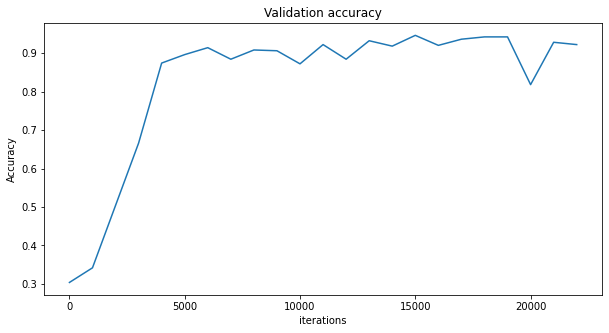
\includegraphics[scale=0.4]{validation_accuracy.png}}
        \caption{Validation accuracy}
        \label{fig:acc}
    \end{subfigure}
    \hfill
    \begin{subfigure}[b]{0.45\textwidth}
        \centerline{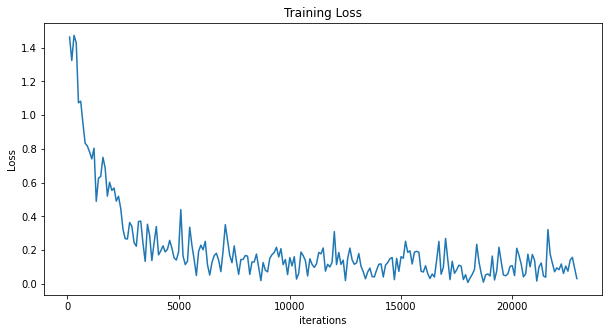
\includegraphics[scale=0.4]{training_loss.png}}
        \caption{Training loss}
        \label{fig:loss}
    \end{subfigure}
    \caption{Multi-digit MNIST octal-division task learning curves: accuracy on the multi-digit test set \ref{fig:acc} and training loss on the single-digit training set \ref{fig:loss}.}
    \label{fig:training_curves}
\end{figure}

% In this section we briefly present the results obtained solving the multi-digit MNIST octal-division task.
In this section, we briefly present the results obtained evaluating the performance of the DeepProbLog framework on the multi-digit MNIST octal-division task.

We trained the model on a training set made of 22,958 pairs and evaluated it on a test set made of 1,462 pairs.
% Our experiments show that DeepProbLog achieves high performance on the multi-digit MNIST octal-division task.
The learning process managed to achieve $97\%$ of accuracy on the test set after around 15,000 iterations as shown in Fig. \ref{fig:acc}. It is worth noting that the process is able to reach a validation accuracy of about $90\%$ after just 5,000 iterations.
% The losses on the training
Fig. \ref{fig:loss} shows the loss obtained on the training set during the learning process: the loss significantly decreases during the first 5,000 iterations and then it tends to oscillate under the value of $0.2$ in agreement with the validation accuracy.
% The learning curve is shown in Fig. \ref{fig:loss}.

This suggests that DeepProbLog is able to effectively leverage the logical rules and the neural network, handling multi-digit numbers in the test set without being explicitly trained on them, converging faster and requiring a smaller training set compared to traditional neural network models. These results demonstrates the effectiveness of DeepProbLog in solving challenging Deep Learning problems.
